
\texcolor{red}{STA ROBA NON È DA INCLUDERE}


\paragraph{Progettazione di dettaglio}
	\subparagraph{Suddivisione lavoro}\Spazio
	\begin{table}[H]
	\centering
	\begin{tabular}{|C{4.5cm}|C{1cm}|C{1cm}|C{1cm}|C{1cm}|C{1cm}|C{1cm}|C{3cm}|}
		\hlineB{3}
		\thead{Nominativo} &\thead{Pm} &\thead{Am} &\thead{An}&\thead{Pt}&\thead{Pr}&\thead{Ve}&\thead{Ore totali}\\
		\hlineB{3}
		Paolo Eccher      & - & - & - & 18(-5) & - & 5(+5) & 23 \\
		\hline
		Alberto Gallinaro & 6 & - & - & 16 & - & 2 & 24 \\
		\hline
		Giuseppe Merlino  & - & - & - & 2 & - & 20 & 22 \\
		\hline
		Elia Montecchio   & 2 & - & - & 5(+5) & - & 17(-5) & 24 \\
		\hline
		Lisa Parma        & - & 3 & - & 20 & - & 0 & 23 \\
		\hline
		Francesco Parolini& - & - & - & 17 & - & 6 & 23 \\
		\hline
		Davide Zago       & - & 4 & - & 13 (-1) & - & 5 & 22 \\
		\hline
		\textbf{Ore totali ruolo}  & \textbf{8} & \textbf{7} & \textbf{-} & \textbf{91(-1)} & \textbf{-} & \textbf{55} & \textbf{161(-1)} \\
		\hlineB{3}
	\end{tabular}
	\caption{Nuova suddivisione del lavoro - \textit{Progettazione di dettaglio}}
\end{table}

Tali dati sono riassunti graficamente nel seguente diagramma a barre:
\begin{figure}[H] 
	\centering 
	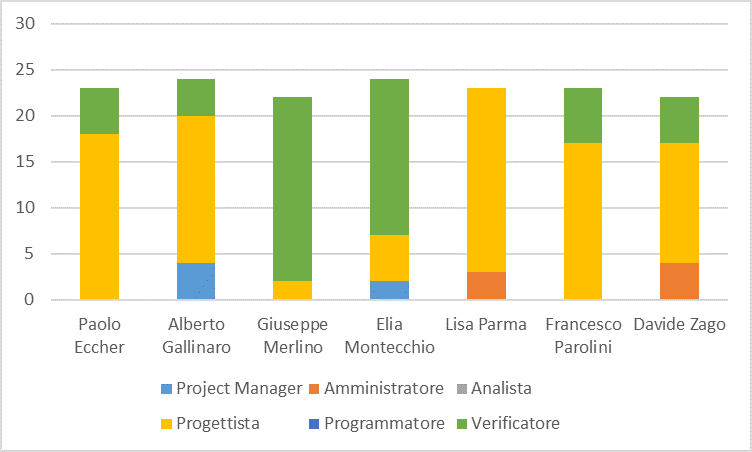
\includegraphics[width=0.9\textwidth]{images/BarreProgettazioneDiDettaglioNuova.png} 
	\caption{Nuova suddivisione ruoli per persona - \textit{Progettazione di Dettaglio}}
	\label{BarreProgettazioneDiDettaglio}
\end{figure}

\subparagraph{Prospetto economico} \Spazio
Nello svolgimento di questa attività i costi sostenuti per ogni ruolo sono riassunti nella seguente tabella:
\begin{table}[H]
	\centering
	\begin{tabular}{|p{4cm}|C{4cm}|C{4cm}|}
		\hlineB{3}
		
		\thead{Ruolo} &\thead{Ore previste} &\thead{Costo}\\
		\hlineB{3}			
		Project Manager & 8 & 240,00\euro \\
		\hline
		Amministratore& 7 & 140,00\euro \\
		\hline
		Analista & - & 0\euro \\
		\hline
		Progettista & 91 (-1) & 2.002,00\euro \\
		\hline
		Programmatore & - & 0\euro \\
		\hline
		Verificatore & 55 & 825,00\euro \\
		\hline
		\textbf{Ore totali} & \textbf{162} & \textbf{3.207,00 \euro} \\
		\hlineB{3}
	\end{tabular}
	\caption{Costi per ruolo - \textit{Progettazione di Dettaglio}}
\end{table}

La ripartizione delle ore tra i vari ruoli è rappresentata graficamente tramite il seguente diagramma circolare:

\begin{figure}[H] 
	\centering 
	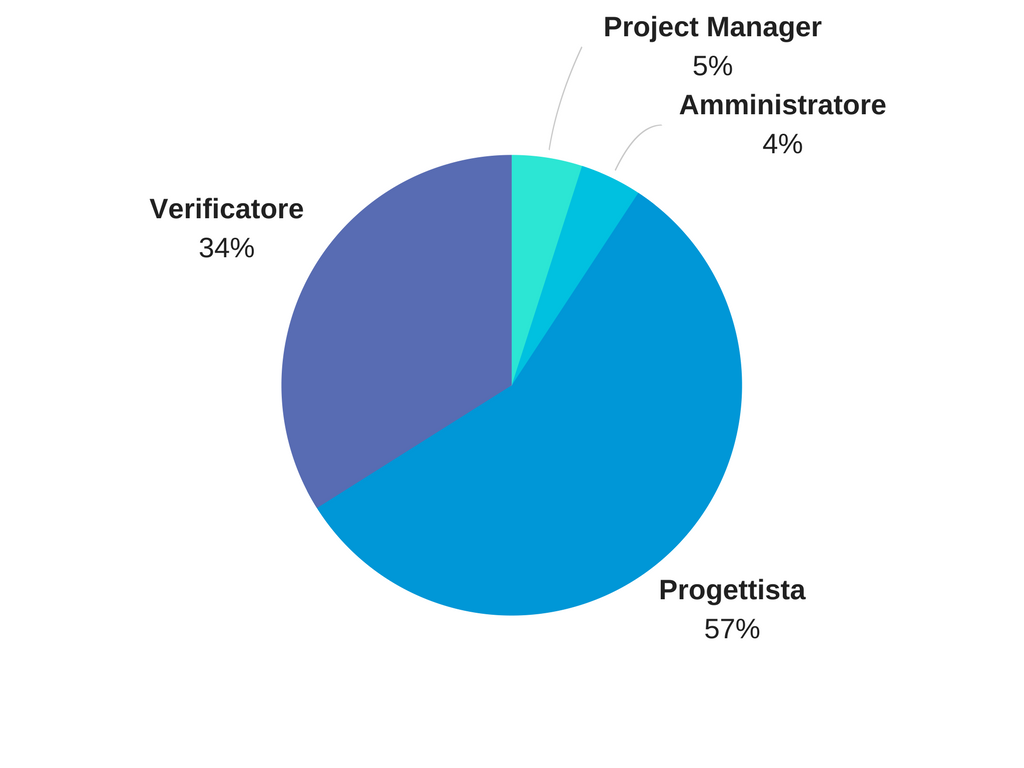
\includegraphics[width=0.9\textwidth]{images/CircolareProgettazioneDiDettaglioNuova.png} 
	\caption{Diagramma circolare ripartizione ore per ruolo in Progettazione di Dettaglio}
	\label{CircolareProgettazioneDiDettaglio}
\end{figure}


\paragraph{Codifica}\Spazio
	\subparagraph{Suddivisione lavoro} \Spazio
	Nell'attività di \textit{Codifica} ciascun componente andrà a rivestire i seguenti ruoli:
	\begin{table}[H]
		\centering
		\begin{tabular}{|C{4cm}|C{0.8cm}|C{0.8cm}|C{0.8cm}|C{0.9cm}|C{0.9cm}|C{0.8cm}|C{2.5cm}|}
			\hlineB{3}
			\thead{Nominativo} &\thead{Pm} &\thead{Am} &\thead{An}&\thead{Pt}&\thead{Pr}&\thead{Ve}&\thead{Ore totali}\\
			\hlineB{3}
			Paolo Eccher      & - & - & - & 15 (+5) & 5 (-5) & 13 & 33 \\
			\hline
			Alberto Gallinaro & 4 (-1) & - & - & 14 (+4) & 14 (-4) & - & 32 \\
			\hline
			Giuseppe Merlino  & - & 6 & - & - & 28 & - & 34 \\
			\hline
			Elia Montecchio   & - & - & - & 8 & 6 (-7) & 20 & 34 (+1) \\
			\hline
			Lisa Parma        & - & - & - & - & 13 & 20 & 33 \\
			\hline
			Francesco Parolini& - & - & - & 11 (+4) & 18 & 9 & 35 (+1) \\
			\hline
			Davide Zago       & 5 (-1) & - & - & 10 (+10) & 10 (-10) & 8 & 33 \\
			\hline
			\textbf{Ore totali ruolo}  & \textbf{9 (-2)} & \textbf{6} & \textbf{-} & \textbf{58} & \textbf{91} & \textbf{70} & \textbf{234 (-2)} \\
			\hlineB{3}
		\end{tabular}
		\caption{Nuova suddivisione del lavoro - \textit{Codifica}}
	\end{table}
	
	Tali dati sono riassunti graficamente nel seguente diagramma a barre:

	\begin{figure}[H] 
		\centering 
		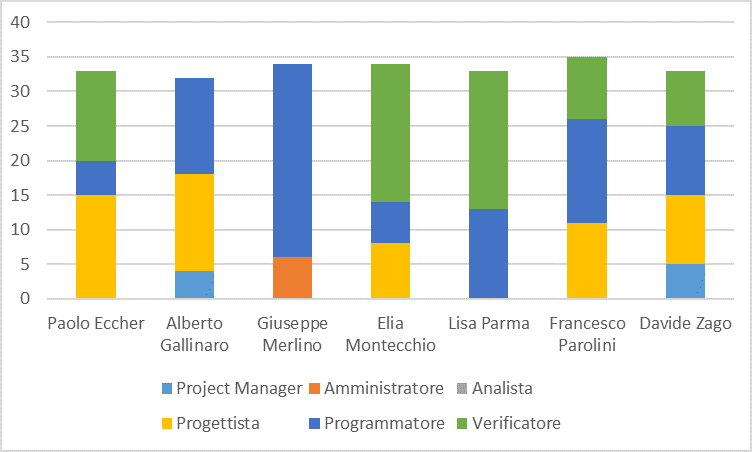
\includegraphics[width=0.9\textwidth]{images/BarreCodificaNuova.png} 
		\caption{Nuova suddivisione ruoli per persona - \textit{Codifica}}
		\label{BarreCodifica}
	\end{figure}
	
	\subparagraph{Prospetto economico} \Spazio
	Nello svolgimento di questa attività i costi sostenuti per ogni ruolo sono riassunti nella seguente tabella:
	\begin{table}[H]
		\centering
		\begin{tabular}{|p{4cm}|C{4cm}|C{4cm}|}
			\hlineB{3}
			
			\thead{Ruolo} &\thead{Ore previste} &\thead{Costo}\\
			\hlineB{3}			
			Project Manager & 9 (-2) & 270,00\euro \\
			\hline
			Amministratore& 6 & 120,00\euro \\
			\hline
			Analista & - & 0\euro \\
			\hline
			Progettista & 58 (+31) & 1.276,00\euro \\
			\hline
			Programmatore & 91 (-29) & 1.365,00\euro \\
			\hline
			Verificatore & 70 & 1.050,00\euro \\
			\hline
			\textbf{Ore totali} & \textbf{234} & \textbf{4.141,00\euro(+187,00\euro )} \\
			\hlineB{3}
		\end{tabular}
		\caption{Costi per ruolo - \textit{Codifica}}
	\end{table}
	
	La ripartizione delle ore tra i vari ruoli è rappresentata graficamente tramite il seguente diagramma circolare:
	
	\begin{figure}[H] 
		\centering 
		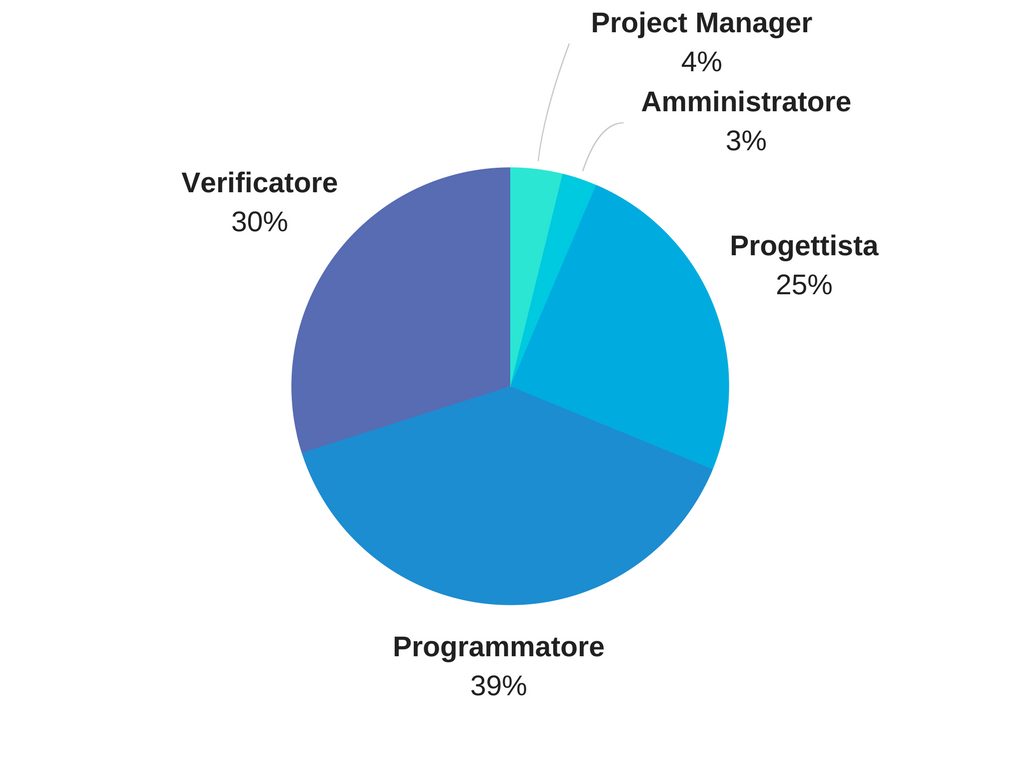
\includegraphics[width=0.9\textwidth]{images/CircolareCodificaNuova.png} 
		\caption{Diagramma circolare ripartizione ore per ruolo in Codifica}
		\label{CircolareCodifica}
	\end{figure}

	


\paragraph{Validazione}
\subparagraph{Suddivisione lavoro} \Spazio
\begin{table}[H]
	\centering
	\begin{tabular}{|C{4cm}|C{1cm}|C{0.6cm}|C{0.6cm}|C{1.5cm}|C{0.6cm}|C{0.6cm}|C{3cm}|}
		\hlineB{3}
		\thead{Nominativo} &\thead{Pm} &\thead{Am} &\thead{An}&\thead{Pt}&\thead{Pr}&\thead{Ve}&\thead{Ore totali}\\
		\hlineB{3}
		Paolo Eccher       & - & - & - & 2 & - & 15 & 17 \\
		\hline
		Alberto Gallinaro  & - & 3 & - & - & - & 14 & 17 \\
		\hline
		Giuseppe Merlino   & - & - & - & 5 & - & 12 & 17 \\
		\hline
		Elia Montecchio    & - & - & - & 9 & - & 10 & 19 \\
		\hline
		Lisa Parma         & - & - & - & 10 & - & 7 & 17 \\
		\hline
		Francesco Parolini & 2 & - & - & - & - & 15 & 17 \\
		\hline
		Davide Zago        & 4(-2) & - & - & 2(+2) & - & 12 & 20(+2) \\
		\hline
		\textbf{Ore totali ruolo}  & \textbf{8} & \textbf{3} & \textbf{-} & \textbf{28(+2)} & \textbf{-} & \textbf{85} & \textbf{124(+4)} \\
		\hlineB{3}
	\end{tabular}
	\caption{Nuova suddivisione del lavoro - \textit{Validazione}}
\end{table}

Tali dati sono riassunti graficamente nel seguente diagramma a barre:

\begin{figure}[H] 
	\centering 
	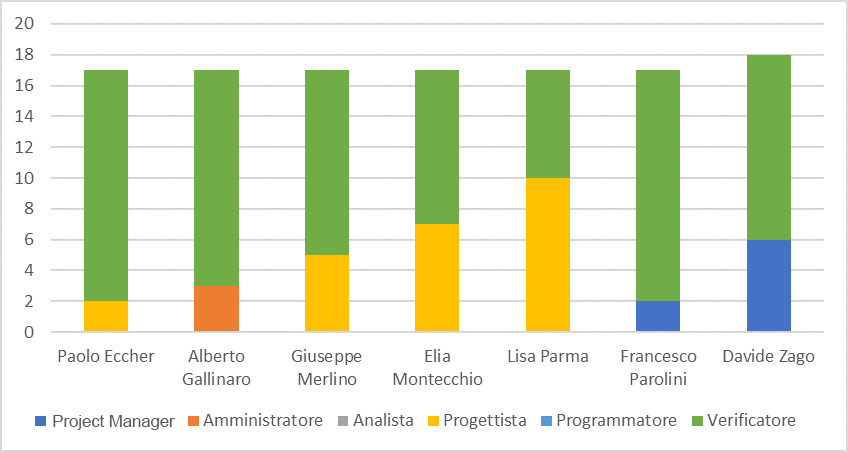
\includegraphics[width=0.9\textwidth]{images/BarreValidazioneNuova.png} 
	\caption{Suddivisione ruoli per persona - \textit{Validazione}}
	\label{BarreValidazione}
\end{figure}

\paragraph{Prospetto economico}	\Spazio
Nello svolgimento di questa attività i costi sostenuti per ogni ruolo sono riassunti nella seguente tabella:
\begin{table}[H]
	\centering
	\begin{tabular}{|p{4cm}|C{4cm}|C{4cm}|}
		\hlineB{3}
		
		\thead{Ruolo} &\thead{Ore previste} &\thead{Costo}\\
		\hlineB{3}			
		Project Manager & 6 & 180,00\euro \\
		\hline
		Amministratore& 3 & 60,00\euro \\
		\hline
		Analista & - & 0\euro \\
		\hline
		Progettista & 28 (+8) & 616,00\euro (+88\euro) \\
		\hline
		Programmatore & - & 0,00\euro \\
		\hline
		Verificatore & 87 (+2) & 1.305,00\euro (+30\euro) \\
		\hline
		\textbf{Ore totali} & \textbf{102} & \textbf{2.191,00\euro(+118\euro)} \\
		\hlineB{3}
	\end{tabular}
	\caption{Costi per ruolo - \textit{Validazione}}
\end{table}

La ripartizione delle ore tra i vari ruoli è rappresentata graficamente tramite il seguente diagramma circolare:
\begin{figure}[H] 
	\centering 
	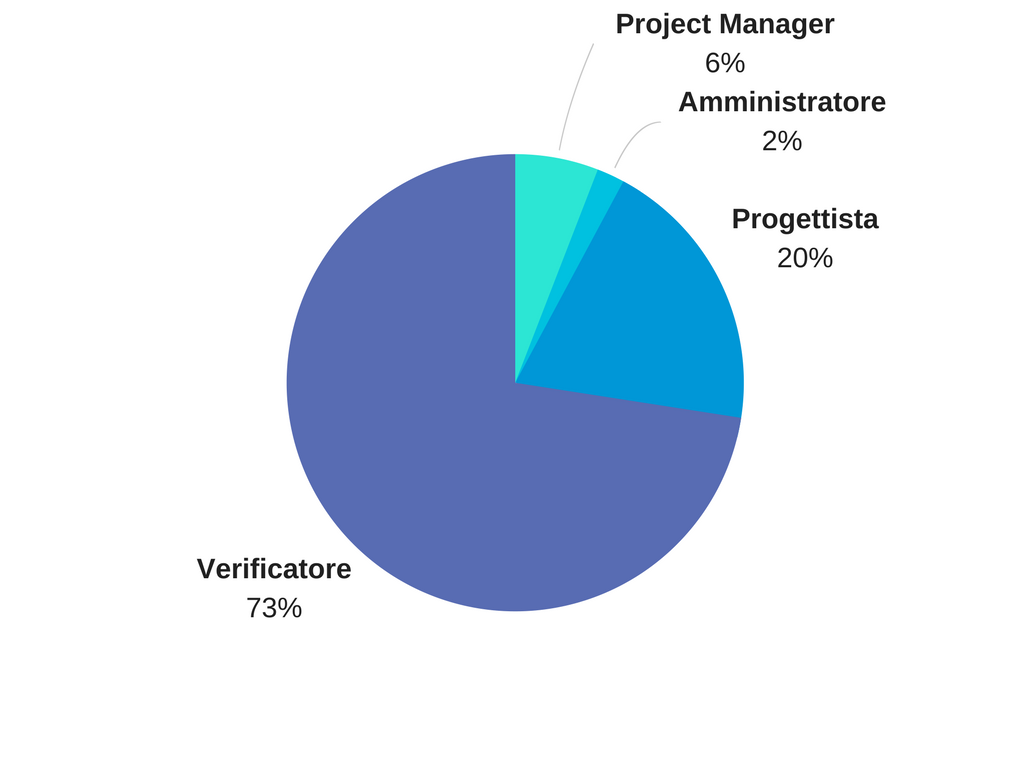
\includegraphics[width=0.9\textwidth]{images/CircolareValidazioneNuova.png} 
	\caption{Diagramma circolare ripartizione ore per ruolo in Validazione}
	\label{CircolareValidazione}
\end{figure}

Il totale delle ore rendicontate diventa quindi il seguente:
			\begin{table}[H]
	\centering
	\begin{tabular}{|C{4cm}|C{0.8cm}|C{0.8cm}|C{0.8cm}|C{0.8cm}|C{0.8cm}|C{0.8cm}|C{3cm}|}
		\hlineB{3}
		\thead{Nominativo} &\thead{Pm} &\thead{Am} &\thead{An}&\thead{Pt}&\thead{Pr}&\thead{Ve}&\thead{Ore totali}\\
		\hlineB{3}
		Paolo Eccher       & 5 (-1) & 3 & 3 & 39 (-5) & 17 (+7) & 39 & 106 (+1) \\
		\hline
		Alberto Gallinaro  & 8 (-3) & 6 & 4 & 38 (-5) & 24 (+6) & 23 & 106 (+1) \\
		\hline
		Giuseppe Merlino   & 0 & 6 & 4 & 17 (-5) & 34 (+6) & 45 & 106 (+1) \\
		\hline
		Elia Montecchio    & 5 & 0 & 3 & 32 (+8) & 6 (-7) & 60 & 106 (+1) \\
		\hline
		Lisa Parma         & 8 (+1) & 3 & 0 & 46 & 13 & 36 & 106 (+1) \\
		\hline
		Francesco Parolini& 6 & 5 & 2 & 36 (+2) & 23 (+5) & 34 (-6) & 106 (+1) \\
		\hline
		Davide Zago        & 12 & 4 & 3 & 32 & 10 (-10) & 42 (+8) & 106 (+1) \\
		\hline
		\textbf{Ore totali ruolo}  & \textbf{44 (-3)} & \textbf{27} & \textbf{19} & \textbf{240 (-5)} & \textbf{127 (+7)} & \textbf{283 (+5)} & \textbf{740 (+5)} \\
		\hlineB{3}
	\end{tabular}
	\caption{Nuova suddivisione del lavoro - Ore rendicontate }
\end{table}

Tali dati sono riassunti graficamente nel seguente diagramma a barre:
\begin{figure}[H] 
	\centering 
	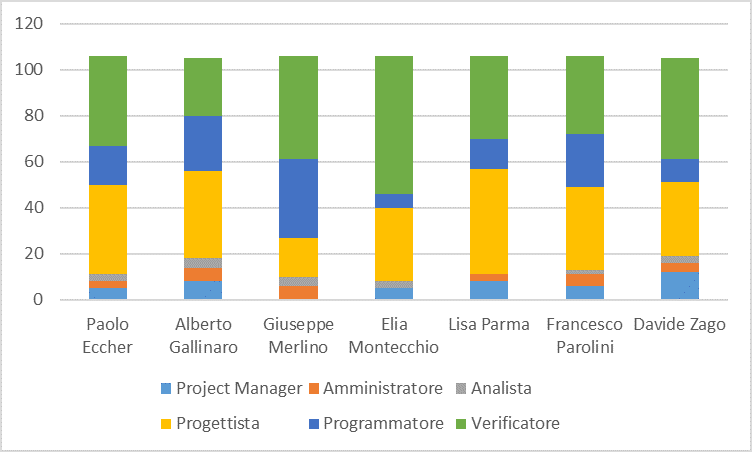
\includegraphics[width=0.9\textwidth]{images/BarreSoloRendicontatoNuovo.png} 
	\caption{Nuova suddivisione ore per ogni ruolo per persona - \textit{Ore rendicontate}}
	\label{BarreRendicontate}
\end{figure}

Il totale rendicontato dei costi sostenuti per ogni ruolo è riassunto nella seguente tabella:
\begin{table}[H]
	\centering
	\begin{tabular}{|p{4cm}|C{4cm}|C{4cm}|}
		\hlineB{3}
		
		\thead{Ruolo} &\thead{Ore previste} &\thead{Costo}\\
		\hlineB{3}			
		Project Manager & 44 (-3) & 1.320,00\euro (-90,00\euro) \\
		\hline
		Amministratore& 27 & 540,00\euro \\
		\hline
		Analista & 19 & 475,0\euro \\
		\hline
		Progettista & 240 (-5) & 5.280,00\euro (-110,00\euro) \\
		\hline
		Programmatore & 127 (+7) & 1.905,00\euro (+105,00\euro) \\
		\hline
		Verificatore & 283 (+6) & 4.245,00\euro (+90,00\euro)\\
		\hline
		\textbf{Ore totali} & \textbf{740(+5)} & \textbf{13.765,00 \euro (-5\euro)} \\
		\hlineB{3}
	\end{tabular}
	\caption{Costi per ruolo - Ore rendicontate}
\end{table}

La ripartizione delle ore tra i vari ruoli è rappresentata graficamente attraverso il seguente diagramma circolare:

\begin{figure}[H] 
	\centering 
	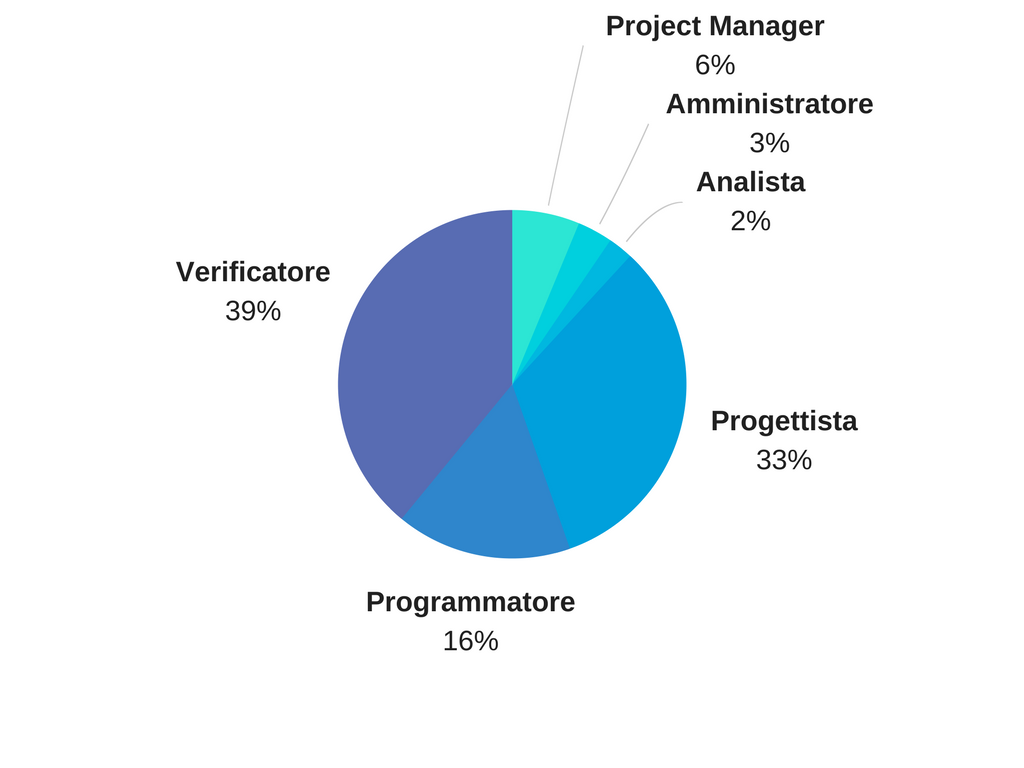
\includegraphics[width=0.9\textwidth]{images/CircolareSoloRendicontateNuovo.png} 
	\caption{Diagramma circolare ripartizione ore rendicontate per ruolo}
	\label{CircolareSoloRendicontate}
\end{figure}

Il bilancio finale aggiornato risulta essere \textbf{13.765,00\euro}. Esso è di 5\euro inferiore rispetto al precedente nonostante vi siano 5 ore in più di lavoro.
